\documentclass[12pt]{article}

\usepackage[english]{babel}
\usepackage[utf8]{inputenc}
\usepackage[top=2cm, left=2cm, right=2cm, bottom=2cm]{geometry}
\usepackage{minted,times,graphicx,fontspec}
\usepackage[slantfont,boldfont]{xeCJK}
\PassOptionsToPackage{hyphens}{url}\usepackage{hyperref}

\setlength\parindent{0pt}
\sloppy
\usemintedstyle{vs}

\title{COMP SCI 7412 Secure Software Engineering Assignment 2}
\author{Tinson Lai \\ a1812422}
\date{}

\begin{document}

\maketitle

\section{Part 2}

\subsection{meetecho/janus-gateway}

Repository: meetecho/janus-gateway

Commit: 3f41a662f4fd4f00b90c307678211fd94f90e103

Stars: ~4.6k

Contributors: 194

File: rtp.c

Language: C

CVE ID: CVE-2020-14034

CWE ID: 120 (Classic Buffer Overflow => Code Injection + (potentially) Arc Injection)

Lines: 94

Fix: dacb4edfad8e77f73b64d8c175cca0a7796ebf80

Comments: This is a typical example of misusing \mintinline{c}|sscanf|. A malicious attack can be launched by crafting a long extension (over 99 characters in this circumstance) in the request. This will also provide a better environment for arc injection attack based on code injection since the succeeding address for overflow is predictable and fixed (local stack variable). It will be easier to inject malicious flow controls. The fix imposed later has solved this problem by simply restricting the length to a constant number, it can then guarantee it will not write to memory region out of the allocated space. This is also the most common way to avoid buffer overflow.

\subsection{netdata/netdata}

Repository: netdata/netdata

Commit: a35bd00fbf8f2578ec0c660b532e925911191b43

Stars: ~49k

Contributors: 411

File: web/api/web\_api\_v1.c

Language: C

CVE ID: CVE-2018-18836

CWE ID: CWE-94 (Code Injection)

Lines: 380-382

Fix: 92327c9ec211bd1616315abcb255861b130b97ca

Comments: A malicious client can launch an attack to update values within the database. This can be achieved by adding commas or some special characters inside the request which will change the JSON string to a different unexpected content. In its fixing commit, the contributor add an extra sttep of filtering out special characters so that only alphanumeric characters will be kept inside the received parameters, and actually, neutralisation in the fixing commit is the most common way to prevent this kind of flaw.

\subsection{LibVNC/libvncserver}

Repository: LibVNC/libvncserver

Commit: 4616de68e664a8136b16c3003d33ba37d0438df3

Stars: 655

Contributors: 71

File: libvncserver/rre.c

Language: C

CVE ID: CVE-2020-14404

CWE ID: 119 (Improper Restriction of Operations within the Bounds of a Memory Buffer)

Comments: This is actually a minor bug since the bound checking should always be inserted before the operation but no after the operation. This bug appears to be an accidental mistake but not a conceptual error from my perspective. Anyway, the fixing commit has corrected the order of operations in the condition. This will only affect the integrity of the software since the bug will potentially crash the program.

\subsection{Summary}

Honestly, I've been using C++ (so as C) for around ten years. Careful handling of low-level system details is always the focused topic. Although most of the C++ language features has enhanced the protection from the language design level, considering the interoperability with C and Assembly, it is still more vulnerable than other interpreter-based or VM-based languages. It is really a basic manner to (correctly) add bound checking to most of the uncertain operations to these two languages, or otherwise, segmentation fault is usually the best circumstance it could happen. What even worse is data breaches or unauthorised executions.

\section{Part 3}

\subsection{ex1}

\subsubsection{Original}

\inputminted{text}{exercise/ex1.enc}

\subsubsection{Decrypted}

\inputminted{text}{exercise/ex1.dec}

\subsubsection{Steps}

It involves multiple guesses. First, this is obviously a letter, thus we can infer that

\begin{itemize}
  \item \mintinline{text}|fc| is \mintinline{text}|hi|
  \item \mintinline{text}|kfggxt| is \mintinline{text}|cheers|
\end{itemize}

Based on the first inference, we can further deduce that

\begin{itemize}
  \item \mintinline{text}|fow| is \mintinline{text}|how|
  \item \mintinline{text}|nxg| is \mintinline{text}|are|
  \item \mintinline{text}|qoa| is \mintinline{text}|you|
  \item \mintinline{text}|ixgg| is \mintinline{text}|free|
  \item \mintinline{text}|dfct| is \mintinline{text}|this|
  \item \mintinline{text}|ixcjnq| is \mintinline{text}|friday|
  \item \mintinline{text}|sczfd| is \mintinline{text}|night|
\end{itemize}

Eventually, we can solve the rest of the unknown characters

\begin{itemize}
  \item \mintinline{text}|hoh| is \mintinline{text}|bob|
  \item \mintinline{text}|grgxqdfcsz| is \mintinline{text}|everything|
  \item \mintinline{text}|pbnsscsz| is \mintinline{text}|planning|
  \item \mintinline{text}|loxg| is \mintinline{text}|more|
\end{itemize}

Then all used characters and words are decrypted. There are some characters were not presented in the text, so the eventual ciphertext key may have numerous possibilities. The replacement is done by a script:

\inputminted{python}{exercise/ex1_dec.py}

\subsection{ex2}

This part is a bit tricky. Based on the hint, I used a script to enumerate all possible weekday name and the encrypted word with matching lengths:

\inputminted{python}{exercise/ex2_enum.py}

The result is:

\inputminted{text}{exercise/ex2_enum.result}

So the key should be \mintinline{text}|ecms|. By writing another simple script:

\inputminted{python}{exercise/ex2_dec.py}

It is obvious that the original message is:

\inputminted{text}{exercise/ex2.dec}

\subsection{ex3}

According to the hint, the cracking can be done by (run for around 2 seconds on my desktop):

\inputminted{python}{exercise/ex3_crack.py}

And the plain text is \mintinline{text}|sun|.

\section{Part 4}

As a Chinese, I think the following IMEs will be more or less familiar to us:

\begin{itemize}
  \item Baidu Pinyin (百度输入法)
  \item Sogou Pinyin (搜狗输入法)
  \item QQ Pinyin from Tencent (QQ拼音)
  \item etc.
\end{itemize}

And actually, for faster typing, some may also learn to use Wubi (五笔, namely, five-strokes, a shape-based input method), but I just hate this since it needs so much memorisation. I am using none of these third-party IMEs. In fact, I have three types of devices in use:

\begin{itemize}
  \item Apple iOS
  \item Microsoft Windows
  \item Google Android
\end{itemize}

I also used to have Ubuntu with KDE Plasma installed on my desktop, but I deleted that several months ago since its performance doesn't differ too much from WSL (Windows Subsystem for Linux). As far as I know, there is a third-party IME for Linux called \mintinline{text}|fcitx| (小企鹅输入法) and its newer version \mintinline{text}|fcitx-5|. I haven't installed any third-party IMEs for around 6 years since Microsoft has incorporated and enhanced their own IME starting from Windows 8. Currently, what I am using is

\begin{itemize}
  \item Microsoft Pinyin for Windows
  \item Google Keyboard (Pinyin) for Android
  \item Apple Pinyin for iOS \& macOS
  \item \mintinline{text}|fcitx| as mentioned.
\end{itemize}

Thus I don't have any third-party privacy concerns. However, a potential privacy concern here is that the built-in IME will also share its data to the other departments within the same corporation, for instance, search engines like Google or Bing. Apple doesn't participate in the search engines competition, but it uses these data to improve suggestions made by Siri as Apple claimed. Apple has been criticised for their poor privacy protection with respect to data on Siri, and the most recent scandal occurred in 2019\footnote{\url{https://www.forbes.com/sites/jeanbaptiste/2019/07/30/confirmed-apple-caught-in-siri-privacy-scandal-let-contractors-listen-to-private-voice-recordings/\#4034d3f57314}}. Google has a data breach scandal in 2018, and it has been criticised on covering up the discovery of the bug which causes the data leakage\footnote{\url{https://www.wsj.com/articles/google-exposed-user-data-feared-repercussions-of-disclosing-to-public-1539017194}}. Generally, however, most of the privacy concern is more relative to Android system, as pointed out in the given reference\footnote{\url{https://doi.org/10.1145/2666356.2594299}}.

\subsection{\mintinline{text}|fcitx|}

The IME, \mintinline{text}|fcitx|, is an open-source project\footnote{\url{https://github.com/fcitx}} initially created by a Chinese C++ programmer. It is only an IME engine in lieu of the native \mintinline{text}|ibus| available on most of the Linux distributions. Basically, it has three different add-ons for the actual typing,

\begin{itemize}
  \item \mintinline{text}|fcitx-cloudpinyin| uses the Baidu Pinyin
  \item \mintinline{text}|fcitx-sunpinyin| uses the open-source statistical language model \mintinline{text}|sunpinyin|\footnote{\url{https://github.com/sunpinyin/sunpinyin}}
  \item \mintinline{text}|fcitx-googlepinyin| uses the cloud-based Google Pinyin service\footnote{\url{https://www.google.com/inputtools/services/features/input-method.html}}
\end{itemize}

Since the development progress of Pinyin on Linux is very slow, none of these has the ability to perform cloud synchronisation.

\subsection{Microsoft/Google/Apple Pinyin}

A general concern amongst these big companies is that they will use data recorded from their own IME input methods to improve their services, and they will also supply these data to other components within the ecosystem they built. They also try to fetch user's personal data from both the running devices and the associated account, such as contacts or emails, to enhance the user experience of the input method. They will also stored custom phrases input by the user into a dictionary, which will potentially be synchronised to the cloud so that it can be accessed across devices. All of these data collected by each company will form a unique identity of the user in their own ecosystem. A data breach will, therefore, easily expose these data. \\

Another potential way of leaking data is that, due to the evolution of modern Machine Learning, most of the phrases will not only be recorded but also fed to their machine learning model for phrase candidates ranking. This indeed encourages the development of the modern smart Pinyin, which greatly improves the user experience. The negative effect is that it will also expose certain characteristics of the user. \\

Let's pretend a user called San Zhang (张三). He may try to shorten the typing to simply 'z' then 's' when he tries to type his name because of the support of smart (ML-based) fuzzy Pinyin. On my desktop (Windows), it will be something like:

\begin{figure}[H]
  \centering
  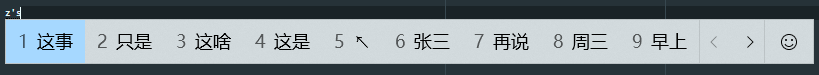
\includegraphics[scale=0.6]{zs.png}
\end{figure}

Since I just typed this word, it is even now ranked higher than most of the other common words. If the user itself type this shorthand will usually get his name as the first choice amongst the candidates. Similarly, some specific terminologies within some specific fields (such as Computer Science) which less frequently appears in daily life will potentially reflect the characteristics such as jobs etc. of the user.

\end{document}
